\documentclass[a4paper,8pt,landscape]{extarticle}

% PARAMETER TO GREY OUT TEXT
\usepackage{etoolbox}
\newtoggle{greytext}
%\toggletrue{greytext}
\togglefalse{greytext}

% paper layout
\usepackage[margin=0.25cm]{geometry}

% page numbers
%\usepackage{fancyhdr}
%\pagestyle{fancy}
%\fancyfoot[R]{\vspace{-38pt}\Large\thepage}

% multicolumn layout
\usepackage{multicol}
\setlength\columnsep{10pt}
\setlength{\columnseprule}{0.1pt} 

% landscape
\usepackage{pdflscape}

% paragraph layout
\setlength\parindent{0pt}
%\setlength\parskip{2pt}

% language settings
%\usepackage[ngerman]{babel} % Silbentrennung (und Deutsche Titel)
\usepackage[utf8]{inputenc} % Umlaute

% font settings
%\usepackage{mathpazo}
%\usepackage{helvet}
%\usepackage{fouriernc}
%\usepackage[varg]{txfonts}
%\usepackage{mathptmx}
%\usepackage[charter]{mathdesign}
%\usepackage[garamond]{mathdesign}
%\usepackage[utopia]{mathdesign}
%\usepackage{fourier}

% font kerning (load after specific font!)
\usepackage{microtype}

% custom font sizes
\usepackage{relsize}

% underlining with line breaks (umlaut support)
%\usepackage{ulem}

% graphics settings
\usepackage{pict2e} % load this before picture
\usepackage{picture}
\usepackage{graphicx}
\usepackage{adjustbox}
\usepackage{caption}
\usepackage{subcaption}

% graphics drawings
\usepackage{tikz}
\usetikzlibrary{calc,matrix,trees,
chains,positioning,decorations.pathreplacing,arrows}
\newcommand{\fadeoutedge}[2]{
\draw (#1) edge ($(#1)!1.8cm!(#2)$) edge [dotted] ($(#1)!2.7cm!(#2)$); 
}
\newcommand{\fadeinedge}[4]{
\draw[<-] (#2) edge ($(#2)!1.8cm!(#1)$) edge [dotted] node
[label_style,#4] {#3} ($(#2)!2.7cm!(#1)$); }
\newcommand{\fadeinoutedge}[4]{
\fadeoutedge{#1}{#2}
\fadeinedge{#1}{#2}{#3}{#4}
}


% plots
\usepackage{pgfplots}

% Set the overall layout of the tree
\tikzstyle{level 1}=[level distance=2cm, sibling distance=2cm]
\tikzstyle{level 2}=[level distance=2cm, sibling distance=1cm]

% Define styles for bags and leafs
\tikzstyle{bag} = [text width=4em, text centered]
\tikzstyle{end} = [circle, minimum width=3pt,fill, inner sep=0pt]

% float settings
\usepackage{float}

% referencing
\usepackage{hyperref}

% math packages and settings
\usepackage{blkarray}  % matrix annotations
\usepackage[intlimits]{mathtools}
\usepackage{amssymb}
\usepackage{wasysym}
\usepackage{dsfont}
\usepackage{resizegather} % resizing equations
\usepackage{oubraces}    % special overlapping over/underbraces
\usepackage{cancel}
\allowdisplaybreaks % allow page break in align* environment

% declares a custom italic bold alphabet for random vectors
\DeclareMathAlphabet{\mathbfit}{OML}{cmm}{b}{it}

% math highlighting
\newcommand{\mathhighlight}[2]{%
  \colorbox{#1}{$\displaystyle#2$}}

\newcommand{\mhlg}[1]{\mathhighlight{green}{#1}}

% tables
\usepackage{booktabs} % nicer tables
\usepackage{array} % custom column types
\usepackage{multirow} % span cells over multiple rows
\newcommand{\tabitem}{~~\llap{{\boldmath $\cdot$}}~} % items in tables

% lists
\usepackage{enumitem}
\setlist{noitemsep,topsep=0pt,parsep=0pt,partopsep=0pt,leftmargin=10pt}

% list items
\renewcommand\labelitemi{{\boldmath$\cdot$}}
\newcommand{\listarrow}{
\smash{\scalebox{1.5}[1.75]{\rotatebox[origin=c]{180}{$\Lsh$}}}
}

% comments (invisible)
\usepackage{comment}

% comments (visible comment)
\newcommand{\txtcom}[1]{\textcolor{gray}{\{ #1 \}}}

\usepackage{dashrule}

% separator
\newcommand{\sep}{\vspace{5pt}\noindent\hrule\vspace{5pt}}

\newcommand{\ssep}{\vspace{2pt}
\begin{tightcenter}\hdashrule[0.5ex]{9cm}{0.1pt}{3mm}
\end{tightcenter}\vspace{2pt}}

% color packages
\usepackage{color}
\usepackage{xcolor}

% color in math (without the bad behaviour of textcolor)
\makeatletter
\def\mathcolor#1#{\@mathcolor{#1}}
\def\@mathcolor#1#2#3{%
  \protect\leavevmode
  \begingroup
    \color#1{#2}#3%
  \endgroup
}
\makeatother

% ASYMPTOTIC NOTATIONS
\newcommand{\BigO}{\mathcal{O}}

% NUMBER SYSTEMS
\newcommand{\E}{\mathbb{E}}
\newcommand{\bbH}{\mathbb{H}}
\newcommand{\K}{\mathbb{K}}
\newcommand{\F}{\mathbb{F}}
\newcommand{\N}{\mathbb{N}}
\newcommand{\Z}{\mathbb{Z}}
\newcommand{\Q}{\mathbb{Q}}
\newcommand{\R}{\mathbb{R}}
\newcommand{\C}{\mathbb{C}}

% CALLICGRAPHIC SHORTCUTS
\newcommand{\cA}{\mathcal{A}}
\newcommand{\cB}{\mathcal{B}}
\newcommand{\cC}{\mathcal{C}}
\newcommand{\cD}{\mathcal{D}}
\newcommand{\cE}{\mathcal{E}}
\newcommand{\cF}{\mathcal{F}}
\newcommand{\cG}{\mathcal{G}}
\newcommand{\cH}{\mathcal{H}}
\newcommand{\cI}{\mathcal{I}}
\newcommand{\cJ}{\mathcal{J}}
\newcommand{\cK}{\mathcal{K}}
\newcommand{\cL}{\mathcal{L}}
\newcommand{\cM}{\mathcal{M}}
\newcommand{\cN}{\mathcal{N}}
\newcommand{\cO}{\mathcal{O}}
\newcommand{\cP}{\mathcal{P}}
\newcommand{\cQ}{\mathcal{Q}}
\newcommand{\cR}{\mathcal{R}}
\newcommand{\cS}{\mathcal{S}}
\newcommand{\cT}{\mathcal{T}}
\newcommand{\cU}{\mathcal{U}}
\newcommand{\cV}{\mathcal{V}}
\newcommand{\cW}{\mathcal{W}}
\newcommand{\cX}{\mathcal{X}}
\newcommand{\cY}{\mathcal{Y}}
\newcommand{\cZ}{\mathcal{Z}}

% SETS
\newcommand{\set}[1]{\left\{ #1 \right\}}
\newcommand{\dset}[2]{\left\{ #1 \ \middle| \ #2 \right\}}

% BRACES
\newcommand{\alg}[1]{\left\langle #1 \right\rangle}
\newcommand{\card}[1]{\left\lvert #1 \right\rvert}
\newcommand{\length}[1]{\left\lvert #1 \right\rvert}
\newcommand{\abs}[1]{\left\lvert #1 \right\rvert}
\newcommand{\norm}[1]{\left\lVert #1 \right\rVert}
\newcommand{\iprod}[1]{\left\langle #1 \right\rangle}
\newcommand{\ceil}[1]{\left\lceil #1 \right\rceil}
\newcommand{\floor}[1]{\left\lfloor #1 \right\rfloor}
\newcommand{\linsys}[2]{\left[\ #1 \ | \ #2 \ \right]}

% BRACES SMALL
\newcommand{\sabs}[1]{\lvert #1 \rvert}
\newcommand{\snorm}[1]{\lVert #1 \rVert}
\newcommand{\siprod}[1]{\langle #1 \rangle}
\newcommand{\slinsys}[2]{[\ #1 \ | \ #2 \ ]}

% DISJOINT UNION
\makeatletter
\def\moverlay{\mathpalette\mov@rlay}
\def\mov@rlay#1#2{\leavevmode\vtop{%
   \baselineskip\z@skip \lineskiplimit-\maxdimen
   \ialign{\hfil$\m@th#1##$\hfil\cr#2\crcr}}}
\newcommand{\charfusion}[3][\mathord]{
    #1{\ifx#1\mathop\vphantom{#2}\fi
        \mathpalette\mov@rlay{#2\cr#3}
      }
    \ifx#1\mathop\expandafter\displaylimits\fi}
\makeatother
\newcommand{\bigcupdot}{\charfusion[\mathop]{\bigcup}{\cdot}}
\newcommand{\cupdot}{\mathbin{\mathaccent\cdot\cup}}

% CUSTOM STATISTICS
\newcommand{\Prob}[2][]{P_{#1}\left( #2 \right)}
\newcommand{\cProb}[2]{P\left( #1 \,\middle|\, #2 \right)}
\newcommand{\hProb}[2][]{\hat{P}_{#1}\left( #2 \right)}
\newcommand{\chProb}[2]{\hat{P}\left( #1 \,\middle|\, #2 \right)}
\newcommand{\Var}[2][]{\operatorname{Var}_{#1}\left[ #2 \right]}
\newcommand{\sd}[1]{\operatorname{sd}\left( #1 \right)}
\newcommand{\Exp}[2][]{{\mathbb{E}_{#1}}\left[ #2
\right]}
\newcommand{\cExp}[3][]{{\mathbb{E}}_{#1}\left[ #2
\,\middle|\, #3 \right]}
\newcommand{\hExp}[2][]{{\mathbb{\hat{E}}_{#1}}\left[ #2
\right]}
\newcommand{\chExp}[3][]{{\mathbb{\hat{E}}}_{#1}\left[ #2
\,\middle|\, #3 \right]}
\newcommand{\Corr}[1]{\operatorname{Corr}\left[ #1 \right]}
\newcommand{\Cov}[1]{\operatorname{Cov}\left(#1 \right)}
\newcommand{\MSE}[2][]{\operatorname{MSE}_{#1}\left[ #2 \right]}
\newcommand{\riid}{\stackrel{\text{\tiny i.i.d.}}{\sim}}
\newcommand{\approxsim}{\stackrel{\text{approx.}}{\sim}}
\newcommand{\ind}[1]{\mathds{1}_{\set{#1}}}

% RANDOM VARIABLES
\newcommand{\rvX}{\mathbfit{X}}

% MACHINE LEARNING
\newcommand{\whR}{\widehat{R}}
\newcommand{\whL}{\widehat{L}}
\newcommand{\whh}{\widehat{h}}
\newcommand{\whP}{\widehat{P}}

% ACCENTS
\newcommand*{\Hm}{\mathsf{H}}
\newcommand*{\T}{\mathsf{T}}
%\newcommand*{\T}{\mkern-1mu{}_{}^{\scriptscriptstyle\top}\mkern-4mu}
\newcommand*{\Rev}{\mathsf{R}}

% CUSTOM ALPHABETS
\renewcommand{\S}{\Sigma}
\newcommand{\Ss}{\Sigma^*}
\newcommand{\Sp}{\Sigma^+}
\newcommand{\Sbool}{\Sigma_{\text{bool}}}
\newcommand{\Ssbool}{(\Sigma_{\text{bool}})^*}
\newcommand{\Slogic}{\Sigma_{\text{logic}}}
\newcommand{\Sslogic}{(\Sigma_{\text{logic}})^*}
\newcommand{\Slat}{\Sigma_{\text{lat}}}
\newcommand{\Sslat}{(\Sigma_{\text{lat}})^*}
\newcommand{\Stastatur}{\Sigma_{\text{Tastatur}}}
\newcommand{\Sstastatur}{(\Sigma_{\text{Tastatur}})^*}
\newcommand{\Sm}{\Sigma_{m}}
\newcommand{\Ssm}{\Sigma_{m}^*}
\newcommand{\ZO}{\{0,1\}}
\newcommand{\ZOs}{\{0,1\}^*}
\newcommand{\hdelta}{\hat\delta}

% OPERATORS
\DeclareMathOperator{\id}{\text{id}}
\DeclareMathOperator{\Kon}{\text{Kon}}
\DeclareMathOperator{\cost}{\text{cost}}
\DeclareMathOperator{\goal}{\text{goal}}
\DeclareMathOperator{\Opt}{\text{Opt}}
\DeclareMathOperator{\Bin}{\text{Bin}}
\DeclareMathOperator{\Nummer}{\text{Nummer}}
\DeclareMathOperator{\Prim}{\text{Prim}}
\DeclareMathOperator{\Kl}{\text{Kl}}
\DeclareMathOperator{\lcm}{lcm}
\DeclareMathOperator{\glb}{glb}
\DeclareMathOperator{\lub}{lub}
\DeclareMathOperator{\im}{im}
\DeclareMathOperator{\ord}{ord}
\DeclareMathOperator{\rank}{rank}
\DeclareMathOperator{\spn}{span}
\DeclareMathOperator{\sign}{sign}
\DeclareMathOperator{\Trace}{Trace}
\DeclareMathOperator{\Count}{Count}
\DeclareMathOperator{\Spur}{Spur}
\DeclareMathOperator{\diag}{diag}
\DeclareMathOperator{\arcsinh}{arcsinh}
\DeclareMathOperator{\arccosh}{arccosh}
\DeclareMathOperator{\arctanh}{arctanh}
% \DeclareMathOperator{\arc}{arc} % TODO: is now a circle of some other package
\renewcommand\div{\operatorname{div}}
\DeclareMathOperator{\rot}{rot}
\DeclareMathOperator{\cis}{cis}
\DeclareMathOperator{\grad}{grad}
\DeclareMathOperator{\Hess}{Hess}
\newcommand{\laplace}{\Delta}
\DeclareMathOperator*{\argmin}{arg\,min}
\DeclareMathOperator*{\argmax}{arg\,max}

% OPERATORS (OVERRIDDEN)
\renewcommand\Re{\operatorname{Re}}
\renewcommand\Im{\operatorname{Im}}

% RELATIONS
\newcommand{\mbeq}{\stackrel{!}{=}}
\newcommand{\relid}{\mathrel{\id}}
\newcommand{\relrho}{\mathrel{\rho}}
\newcommand{\relsigma}{\mathrel{\sigma}}
\newcommand{\reltheta}{\mathrel{\theta}}
\newcommand{\relsim}{\mathrel{\sim}}
\newcommand{\relf}{\mathrel{f}}

% RELATIONS (INVERSES)
\newcommand{\invrelid}{\mathrel{\widehat{\id}}}
\newcommand{\invrelrho}{\mathrel{\widehat{\rho}}}
\newcommand{\invrelsigma}{\mathrel{\widehat{\sigma}}}
\newcommand{\invreltheta}{\mathrel{\widehat{\theta}}}
\newcommand{\invrelsim}{\mathrel{\widehat{\sim}}}
\newcommand{\invrelf}{\mathrel{\widehat{f}}}

% CUSTOM RELATIONS
\DeclareRobustCommand{\step}[2][]{\mathrel{\drawstep{#1}{#2}}}
\newcommand{\drawstep}[2]{%
  \vcenter{\hbox{%
    \setlength{\unitlength}{1em}%
    \begin{picture}(1,1)
    \roundcap
    \put(0,0){\line(0,1){1}}
    \put(0,0.5){\line(1,0){0.95}}
    \put(0.5,0){\makebox[0pt]{\text{\smaller$\scriptscriptstyle#2$}}}
    \put(0.5,0.6){\makebox[0pt]{\text{\smaller$#1$}}}
    \end{picture}%
  }}%
}

% GLOBAL MATRICES AND VECTOR SETTINGS
\newcommand{\boldm}[1] {\mathversion{bold}#1\mathversion{normal}}
\newcommand{\mat}[1]{\mathbf{#1}}
\renewcommand{\vec}[1]{\mathbf{#1}}

% VECTORS
\newcommand{\va}{\vec{a}}
\newcommand{\vb}{\vec{b}}
\newcommand{\vc}{\vec{c}}
\newcommand{\vd}{\vec{d}}
\newcommand{\ve}{\vec{e}}
\newcommand{\vf}{\vec{f}}
\newcommand{\vg}{\vec{g}}
\newcommand{\vh}{\vec{h}}
\newcommand{\vi}{\vec{i}}
\newcommand{\vj}{\vec{j}}
\newcommand{\vk}{\vec{k}}
\newcommand{\vl}{\vec{l}}
\newcommand{\vm}{\vec{m}}
\newcommand{\vn}{\vec{n}}
\newcommand{\vo}{\vec{o}}
\newcommand{\vp}{\vec{p}}
\newcommand{\vq}{\vec{q}}
\newcommand{\vr}{\vec{r}}
\newcommand{\vs}{\vec{s}}
\newcommand{\vt}{\vec{t}}
\newcommand{\vu}{\vec{u}}
\newcommand{\vv}{\vec{v}}
\newcommand{\vw}{\vec{w}}
\newcommand{\vx}{\vec{x}}
\newcommand{\vy}{\vec{y}}
\newcommand{\vz}{\vec{z}}

% VECTORS WITH TILDE ACCENT
\newcommand{\vta}{\widetilde{\vec{a}}}
\newcommand{\vtb}{\widetilde{\vec{b}}}
\newcommand{\vtc}{\widetilde{\vec{c}}}
\newcommand{\vtd}{\widetilde{\vec{d}}}
\newcommand{\vte}{\widetilde{\vec{e}}}
\newcommand{\vtf}{\widetilde{\vec{f}}}
\newcommand{\vtg}{\widetilde{\vec{g}}}
\newcommand{\vth}{\widetilde{\vec{h}}}
\newcommand{\vti}{\widetilde{\vec{i}}}
\newcommand{\vtj}{\widetilde{\vec{j}}}
\newcommand{\vtk}{\widetilde{\vec{k}}}
\newcommand{\vtl}{\widetilde{\vec{l}}}
\newcommand{\vtm}{\widetilde{\vec{m}}}
\newcommand{\vtn}{\widetilde{\vec{n}}}
\newcommand{\vto}{\widetilde{\vec{o}}}
\newcommand{\vtp}{\widetilde{\vec{p}}}
\newcommand{\vtq}{\widetilde{\vec{q}}}
\newcommand{\vtr}{\widetilde{\vec{r}}}
\newcommand{\vts}{\widetilde{\vec{s}}}
\newcommand{\vtt}{\widetilde{\vec{t}}}
\newcommand{\vtu}{\widetilde{\vec{u}}}
\newcommand{\vtv}{\widetilde{\vec{v}}}
\newcommand{\vtw}{\widetilde{\vec{w}}}
\newcommand{\vtx}{\widetilde{\vec{x}}}
\newcommand{\vty}{\widetilde{\vec{y}}}
\newcommand{\vtz}{\widetilde{\vec{z}}}

% VECTORS (GREEK)
\newcommand{\vmu}{\boldsymbol{\mu}}
\newcommand{\valpha}{\boldsymbol{\alpha}}
\newcommand{\vbeta}{\boldsymbol{\beta}}
\newcommand{\vtheta}{\boldsymbol{\theta}}
\newcommand{\vell}{\boldsymbol{\ell}}
\newcommand{\vvarphi}{\boldsymbol{\varphi}}
\newcommand{\vdelta}{\boldsymbol{\delta}}
\newcommand{\vgamma}{\boldsymbol{\gamma}}
\newcommand{\vlambda}{\boldsymbol{\lambda}}

% MATRICES (LATIN)
\newcommand{\MA}{\mat{A}}
\newcommand{\MB}{\mat{B}}
\newcommand{\MC}{\mat{C}}
\newcommand{\MD}{\mat{D}}
\newcommand{\ME}{\mat{E}}
\newcommand{\MF}{\mat{F}}
\newcommand{\MG}{\mat{G}}
\newcommand{\MH}{\mat{H}}
\newcommand{\MI}{\mat{I}}
\newcommand{\MJ}{\mat{J}}
\newcommand{\MK}{\mat{K}}
\newcommand{\ML}{\mat{L}}
\newcommand{\MM}{\mat{M}}
\newcommand{\MN}{\mat{N}}
\newcommand{\MO}{\mat{0}}
\newcommand{\MP}{\mat{P}}
\newcommand{\MQ}{\mat{Q}}
\newcommand{\MR}{\mat{R}}
\newcommand{\MS}{\mat{S}}
\newcommand{\MT}{\mat{T}}
\newcommand{\MU}{\mat{U}}
\newcommand{\MV}{\mat{V}}
\newcommand{\MW}{\mat{W}}
\newcommand{\MX}{\mat{X}}
\newcommand{\MY}{\mat{Y}}
\newcommand{\MZ}{\mat{Z}}

% MATRICES (LATIN) TILDE
\newcommand{\MtA}{\widetilde{\mat{A}}}
\newcommand{\MtB}{\widetilde{\mat{B}}}
\newcommand{\MtC}{\widetilde{\mat{C}}}
\newcommand{\MtD}{\widetilde{\mat{D}}}
\newcommand{\MtE}{\widetilde{\mat{E}}}
\newcommand{\MtF}{\widetilde{\mat{F}}}
\newcommand{\MtG}{\widetilde{\mat{G}}}
\newcommand{\MtH}{\widetilde{\mat{H}}}
\newcommand{\MtI}{\widetilde{\mat{I}}}
\newcommand{\MtJ}{\widetilde{\mat{J}}}
\newcommand{\MtK}{\widetilde{\mat{K}}}
\newcommand{\MtL}{\widetilde{\mat{L}}}
\newcommand{\MtM}{\widetilde{\mat{M}}}
\newcommand{\MtN}{\widetilde{\mat{N}}}
\newcommand{\MtO}{\widetilde{\mat{0}}}
\newcommand{\MtP}{\widetilde{\mat{P}}}
\newcommand{\MtQ}{\widetilde{\mat{Q}}}
\newcommand{\MtR}{\widetilde{\mat{R}}}
\newcommand{\MtS}{\widetilde{\mat{S}}}
\newcommand{\MtT}{\widetilde{\mat{T}}}
\newcommand{\MtU}{\widetilde{\mat{U}}}
\newcommand{\MtV}{\widetilde{\mat{V}}}
\newcommand{\MtW}{\widetilde{\mat{W}}}
\newcommand{\MtX}{\widetilde{\mat{X}}}
\newcommand{\MtY}{\widetilde{\mat{Y}}}
\newcommand{\MtZ}{\widetilde{\mat{Z}}}

% MATRICES (GREEK)
\newcommand{\MSigma}{\mat{\Sigma}}
\newcommand{\MLambda}{\mat{\Lambda}}
\newcommand{\MPhi}{\mat{\Phi}}

\newcommand*{\vertbar}{\rule[-1ex]{0.5pt}{4ex}}
\newcommand*{\horzbar}{\rule[.5ex]{4ex}{0.5pt}}

% HIGHLIGHTING IN EQUATIONS
\newcommand{\hl}[1]{\colorbox{black!7}{$#1$}}

% programming codes
% TODO: use better programming package: pygments
\usepackage{listings}
\usepackage{courier}
\definecolor{light-gray}{gray}{0.9}
\lstset{
 %rulecolor=\color{black},
 %frame=single, % adds a frame around the code
 basicstyle        = \footnotesize\ttfamily,
 framextopmargin   = 50pt
 breaklines        = true,
 breakatwhitespace = true,
 %backgroundcolor=\color{light-gray},
 breakindent       = 2ex,
 escapechar       = *,   % custom escape char
 %numbers          = left
 tabsize           = 2,
 %literate={\ \ }{{\ }}1
 mathescape        = true   % escape math with '$'
}

% todos
\newcommand{\todo}[1]{\textcolor{red}{\textbf{TODO:} #1}}

% TODO: warmup environment (short/long version of document)
% TODO: algorithm package (abstract)
% TODO: graph packages (tikz)
% TODO: minted codes (and language-specific)
% TODO: gnuplot, pgfplots examples
% TODO: displayskip, parskip (what is this?)
% TODO: ultra shortening option for document

% CUSTOM ARGUMENTS
\newcommand{\argdot}{\,\cdot\,}

% custom commands
\include{custom-commands}

% codes
\lstnewenvironment{Code}[1][]{}{}        % boxed
\newcommand{\code}[1]{\lstinline{#1}}    % inline



% title
\title{Learning and Intelligent Systems}
\author{Summary - Summer 2016}
\date{Andreas Bloch}


\iftoggle{greytext}{
% grey out sections
\definecolor{sectioncolor}{rgb}{0.95,0.95,0.95}
\definecolor{sectionbarcolor}{rgb}{0.98,0.98,0.98}
\newcommand*{\mybox}[1]{%
    \noindent\colorbox{sectionbarcolor}{%
        \parbox{\dimexpr\columnwidth-2\fboxsep\relax}{%
            \textcolor{white}{#1}}}}
}{
% use blue color
\definecolor{sectioncolor}{rgb}{0,0,205}
\newcommand*{\mybox}[1]{%
    \noindent\colorbox{sectioncolor}{%
        \parbox{\dimexpr\columnwidth-2\fboxsep\relax}{%
            \textcolor{white}{#1}}}}
}

\usepackage[explicit]{titlesec}
% Raised Rule Command:
% Arg 1 (Optional) - How high to raise the rule
% Arg 2 - Thickness of the rule
\newcommand{\raisedrulefill}[2][0ex]{\leaders\hbox{\rule[#1]{1pt}{#2}}\hfill}
\newcommand{\introrule}[2][0ex]{\leaders\hbox{\rule[#1]{1pt}{#2}}\hfill}

\titleformat{\subsection}{\bfseries}
{\color{sectioncolor}\rule[0.3ex]{5pt}{1.5pt}
\,\thesubsection\,\rule[0.3ex]{8pt}{1.5pt}\,}{0em}
{\color{sectioncolor}#1\,\raisedrulefill[0.3ex]{1.5pt}}
\titleformat{\subsubsection}{\bfseries}
{\color{sectioncolor}\rule[0.35ex]{5pt}{0.5pt}
\,\thesubsubsection\,\rule[0.35ex]{8pt}{0.5pt}\,}{0em}
{\color{sectioncolor}#1\,\raisedrulefill[0.35ex]{0.5pt}}

\titlespacing*{\section}
{0pt}{0ex plus 0ex minus 0ex}{0ex plus 0ex}
\titlespacing*{\subsection}
{0pt}{0ex plus 0ex minus 0ex}{0ex plus 0ex}
\titlespacing*{\subsubsection}
{0pt}{0ex plus 0ex minus 0ex}{0ex plus 0ex}


\makeatletter
\renewcommand\section{\@startsection {section}{1}{\z@}%
                                   {0pt}%
                                   {0pt}%
                                   {\normalfont\bfseries\mybox}}
\makeatother


\newenvironment{tightcenter}{%
  \begin{center}
  \vspace{-4pt}
}{
  \vspace{-4pt}
  \end{center}
}

% remove table of contents title
\makeatletter
\renewcommand\tableofcontents{%
    \@starttoc{toc}%
}
\makeatother

\makeatletter
\setlength{\@fptop}{0pt}
\makeatother

\renewcommand{\baselinestretch}{0.01}



\begin{document}

\small


% reduce spacing in math equations
\setlength{\abovedisplayskip}{0pt}%
\setlength{\belowdisplayskip}{0pt}%
\setlength{\abovedisplayshortskip}{0pt}%
\setlength{\belowdisplayshortskip}{0pt}%
\setlength{\jot}{3pt}% Inter-equation spacing


% define hidden column type for tables
\newcolumntype{H}{>{\setbox0=\hbox\bgroup}c<{\egroup}@{}}

\begin{multicols*}{3}
\raggedcolumns

\iftoggle{greytext}{%
  % grey out text
  \definecolor{lighttext}{rgb}{0.95,0.95,0.95}
  \color{lighttext}
}{
  % show text normel
}

\section{Learning Rates}

Heuristics on how to choose the learning rate:
\begin{itemize}
  \item constant: $\eta_t=10^{-3}$ / decreasing:
  $\eta_t=\max\set{10^{-2},\frac{1}{t}}$
  \item adaptive: $\eta_t = \argmin_\eta \whR(\vw_t-\eta\vg_t)$ \quad (via
  1D-pt. problem)
  \item bold-driver: $\eta_{t+1} := \whR(\vw_{t+1}) < \whR(\vw_t) \ ? \
\eta_{t} \cdot c_{\text{inc}} \ \colon \ \eta_{t-1} \cdot c_{\text{dec}}$
\end{itemize}

\section{Regression}

\subsection{Ridge Regression}

$\vw^*=\argmin_{\vw}\norm{\vy-\MX\vw}_2^2 + \lambda \norm{\vw}_2^2 \qquad
(\lambda > 0, \text{ chosen via CV}) $

\textbf{1) Closed Form} $\BigO(nd^2+d^3)$ (setup + solve)\\ 
$\vw^*=(\MX^\T\MX+\lambda\MI)^{-1}\MX^\T\vy$ \quad (always has a solution)

\textbf{2) Gradient descent} $\BigO(\text{iter.}\times nd)$\\
$\vg_t =-2\MX^\T(\vy-\MX\vw_t) +2\lambda\vw_t$

Note: Now the scale of the data matters for $\lambda$! ($\rightarrow$ normalize
data)

\textbf{1) VS 2)} Complexity, Optimality of Sol., CF possible (enoug data)?

\textbf{Bayesian Interpretation} (=Gaussian MAP) Implicit assumption:
label $y$ is linear in $\vx$, with Gaussian noise with \emph{constant} variance.

$Y\sim\cN(\vw^\T\vx,\sigma^2)$,\quad $y_i=\vw^\T\vx_i+\epsilon$, \quad
$\epsilon\sim\cN(0,\sigma^2)$

$\cProb{Y=y}{\vx=\vx,\vtheta}=\cN(y;h(\vx),\sigma^2)$, \quad 
$h(\vx)=\vw^\T\vx$, \quad
$\vtheta=(\vw,\sigma^2)$

weights prior:
$\vw\sim\cN(0,\beta^2\MI)$,\quad $w_i\sim\cN(0,\beta^2)$

Maximizing $\cProb{\vw}{D}$ then leats to the connection
$\lambda=\frac{\sigma^2}{\beta^2}$.

\subsection{Kernelized Ridge Regression}

\textbf{Insight} optimal $\vw^*$ lies in the span of the data.

$\vw^*=\MX_\phi^\T\vz^*$ \, 
\, ($\MK=\MX_\phi\MX_\phi^\T\in\R^{n\times n}$)

$\vz^*=\argmin_{\vz} \snorm{\MK\vz-\vy}_2^2 + \lambda\vz^\T\MK\vz $

\textbf{1) Closed form} $\vz^*=(\MX_\phi\MX_\phi^\T+\lambda\MI)^{-1}\vy
=(\MK-\lambda\MI)^{-1}\vy$

\textbf{2) Gradient descent} $\vg_t=2\MK^\T(\MK\vz-\vy) + 2 \lambda\MK\vz$

\textbf{Prediction} $f(\vx)={\vw}^\T\phi(\vx)=\ldots=\sum_{i=1}^n
z_ik(\vx_i,\vx)$

\textbf{Bayesian Interpretation} Same as ridge regression, except that the
hypothesis class for $\cH$ for $h$ (comp. of mean) may be different.

\subsection{Sparse Regression: LASSO}

Prior: $w_i\sim p(w_i;0,b)=\frac{1}{2b}e^{-\frac{\abs{w_i-\mu}}{b}}$ where
$\mu=0$, (connection: $\lambda=\frac{2\sigma^2}{b}$).

\subsection{Regression with Outliers}

Use losses smaller than squared loss, or distributions with fatter tails.

\section{Classification}

\subsection{Classification Losses}

\iftoggle{greytext}{
\vspace{70pt}
\textbf{0/1 Loss}
}{
\textbf{0/1 Loss}\qquad
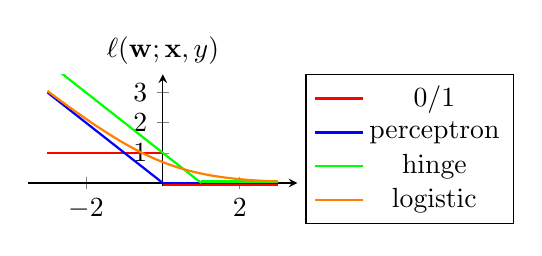
\begin{tikzpicture}
\begin{axis}[
  height = 3cm,
  width = 5cm,
  axis x line=center,
  axis y line=center,
  samples=100,
  xlabel={$y\vw^\T\vx$},
  xlabel style={right},
  ylabel={$\ell(\vw;\vx,y)$},
  ylabel style={above},
  xmin=-3.5,
  xmax=3.5,
  ymin=-0.1,
  ymax=3.6,
  %legend columns=-1,
  legend style={/tikz/every even column/.append style={column sep=0.5cm}},
  legend pos=outer north east
]
  % 0/1 loss
  \addplot[red, thick, domain=-3:0]{1};
  \addplot[red, thick, domain=0:3,forget plot]{-0.05};
  \addlegendentry{0/1}
  % perceptron loss
  \addplot[blue, thick, domain=-3:0]{-x};
  \addplot[blue, thick, domain=0:3,forget plot]{0};
  \addlegendentry{perceptron}
  % hinge loss
  \addplot[green, thick, domain=-3:1]{-x+1};
  \addplot[green, thick, domain=1:3, forget plot]{0.05};
  \addlegendentry{hinge}
  % logistic loss
  \addplot[orange, thick, domain=-3:3]{0.0+(ln(1+e^(-x)))};
  \addlegendentry{logistic}
\end{axis}
\end{tikzpicture}
} 
\begin{gather*}
\begin{align*}
\ell_{0/1}(\vw;\vx,y)=\ind{y_i\neq\sign(\vw^\T\vx)}
=\begin{cases} 
0 &y=\sign(\vw^\T\vx)\\
1 &\text{otherwise}
\end{cases}
=\begin{cases} 
0 &y\sign(\vw^\T\vx)=1\\
1 &\text{otherwise}
\end{cases}
\end{align*} 
\end{gather*}

\subsection{Perceptron}

$\vw^*=\argmin_{\vw}\sum_{i=1}^n \max\set{0,-y_i\vw^\T\vx_i}$

$\vg_t= \sum_{i=1}^n \begin{cases}
0,& -y_i\vw_t^\T\vx_i < 0,\\
-y_i\vx_i,& \text{otherwise}.
\end{cases}
=-\MX^\T\left(\vy\odot\left[-\vy\odot\MX\vw \geq 0\right]\right)
$

\subsection{Kernelized Perceptron}

Ansatz 
$\vw^*=\sum_{j=1}^n 
\alpha_jy_j\phi(\vx_j)=\MX_\phi^\T(\valpha\odot\vy)$
gives:

$
\valpha^*=\argmin_{\valpha}\textstyle\sum_{i=1}^n \max\left(0,
-y_i\valpha^\T\vk_i\right),
$

where $\vk_i=(y_1k(\vx_i,\vx_1),\ldots,y_nk(\vx_i,\vx_n))^\T$.

\textbf{Gradient Step: Equiv. between updating $\vw$ and $\valpha$}\\
\begin{tabular}{ll}
\begin{Code}
if $y_i\vw^\T\vx_i \geq 0$:
  $\vw_t = \vw_{t-1}$
else:
  $\vw_t\leftarrow \vw_{t-1}+\eta_ty_i\phi(\vx_i)$
   = $\sum_{j=1}^n \alpha_j^{(t-1)}y_j\phi(\vx_j)+\eta_ty_i\phi(\vx_i)$
   = $\sum_{j=1}^n \begin{cases}
        \alpha_j^{(t-1)}y_j\phi(\vx_j), & i\neq j\\
        (\alpha_j^{(t-1)}+\eta_t)y_i\phi(\vx_i), &i=j
        \end{cases}$
\end{Code}
&
\begin{Code}
 if $y_i\sum_{j=1}^n\alpha_jy_jk(\vx_i,\vx_j)\geq 0$:
   $\valpha^{(t)} \leftarrow \valpha^{(t-1)}$
 else:
   $\valpha_j^{(t)} \leftarrow \valpha_j^{(t-1)}$ for all $j\neq i$
   $\valpha_i^{(t)} \leftarrow \valpha_i^{(t-1)}+\eta_t$ for $i=j$
\end{Code}\\
\end{tabular}

\textbf{Pred.}
$f(\vx)=\sign\left({\vw^*}^\T\phi(\vx)\right)=\ldots
=\sign\left(\sum_{j=1}^n \alpha_j^* y_jk(\vx_j,\vx)\right)
$

\subsection{Support Vector Machines (SVMs)}

$\vw^*=\argmin_{\vw}\sum_{i=1}^n
\max\set{0,1-y_i\vw^\T\vx_i}+\lambda\norm{\vw}_2^2$ (reg. by default)

Hinge Loss ($\ell_{\text{SVM}}$) maximizes margin of separator.

$\vg_t= \sum_{i=1}^n \begin{cases}
0,& 1-y_i\vw_t^\T\vx_i < 0,\\
-y_i\vx_i,& \text{otherwise}.
\end{cases}+2\lambda\vw_t
$

\quad \ $=-\MX^\T\left(\vy\odot\left[1-\vy\odot\MX\vw \geq 0\right]\right)
+2\lambda\vw_t
$

\subsection{Kernelized Support Vector Machines}

$\valpha^*=\argmin_{\valpha} \sum_{i=1}^n \max\set{0,1-y_i\valpha^\T\vk_i}
+\lambda\valpha^\T\MK\valpha
$

where $\vk_i=(y_1k(\vx_i,\vx_1),\ldots,y_nk(\vx_i,\vx_n))^\T$.

\subsection{Nearest Neighbor Classifiers ($k$-NN)}
$
y=\sign\left(\sum_{i=1}^n y_i\ind{\vx_i \text{ among }k\text{ nearest
neighbors of }\vx}\right)
\,\,
\text{(choose }k\text{ via CV)}
$

\subsection{Logistic Regression}

$\cProb{Y=y}{\vx,\vw}=Ber(y;\sigma(\vw^\T\vx))
=\frac{1}{1+e^{-y\vw^\T\vx}}=p_y$

$\cProb{Y=+1}{\vx,\vw}=\sigma(\vw^\T\vx)=p_+$

Grad. step with Gaussian Prior:
$\vw\leftarrow\vw(1-2\lambda\eta_t) + \eta_t
y\vx \chProb{Y=-y}{\vw,\vx}$

\subsubsection{Multi-Class Logistic Regression}

$\cProb{Y=i}{\vx,\vw_1,\ldots,\vw_c}=\frac{\exp(\vw_i^\T\vx)}{
\sum_{j=1}^c \exp(\vw^\T_j\vx)
}=p_i
$

\section{Kernels}

\subsection{Definition of a Kernel}

For a data space $\cX$	a \emph{kernel} is a function
$k\colon\cX\times\cX\to\R$ satisfying $i)$ and [$ii)$ or $iii)$]:
\begin{enumerate}[label=\roman*)]
  \item \emph{symmetry}: $\forall\vx,\vx'\in\cX\colon k(\vx,\vx')=k(\vx',\vx)$
  \item \emph{positive semi-definiteness}: for any $n$, any set
  $S=\set{\vx_1,\ldots,\vx_n}\subseteq\cX$, the kern G. matrix
  $\MK=[k(\vx_i,\vx_j)]_{1\leq i,j\leq n}$
  must be p. sem. def.
  \item $k$ is an inner product
  $\iprod{\argdot,\argdot}\colon\cF\times\cF\to\R$ in a suitable space 
  $\cF$ (where $\Phi\colon\cX\to\cF$ is the feature map)
\end{enumerate}

\subsection{Common Kernels}

\begin{itemize}
  \item Linear kernel: $k(\vx,\vx')=\vx^\T\vx'$
  \item Monomials of degree $m$: $k(\vx,\vx')=(\vx^\T\vx')^m$
  \item Monomials up to degree $m$: $k(\vx,\vx')=(1+\vx^\T\vx')^m$ 
  \item Gaussian (RBF, Sq. exp. kernel)
  $k(\vx,\vx')=\exp(-\norm{\vx-\vx'}_2^2/h^2)$
  \item Sigmoid (tanh) kernel: $k(\vx,\vx')=\tanh(\kappa\vx^\T\vx')-b$
  \item Laplacian kernel: $k(\vx,\vx')=\exp(-\gamma \norm{\vx-\vx'}_1)$
\end{itemize}

\subsection{Kernel Composition Rules}

$k_1+k_2$ / $k_1\cdot k_2$ / $c\cdot k_1\, (c>0)$ / $f(k_1)$, $f$ poly. pos.
coeff, exponential.

\section{Feature Selection}

\begin{tabular}{@{}ll}
\textbf{Greedy FW} $s_i=\argmin_{j\in V\setminus S} \hat{L}(S\cup\set{j})$
&
\multirow{3}{*}{
\iftoggle{greytext}{
}{
\includegraphics[width=0.15\linewidth]{img/lasso-illustration}
}	
}
\\
\textbf{Greedy BW} $s_i=\argmin_{j\in S} \hat{L}(S\setminus\set{j})$
\\
\textbf{Linear Models:} Sparsity Trick: $\norm{\vw}_0 \to \norm{\vw}_1$
\end{tabular}


\section{Imbalanced Data}

\textbf{Convention:} $+$ is the rare class.

\textbf{Possible Approaches:} Upsampling / Downsampling. Or choosing classifier
based on trade-offs / evaluation metrics:

\textbf{Cost-Sensitive Loss} $R(\vw)=\sum_{i=1}^n
c_{y_i}\min(0,-y_i\vw^\T\vx_i)$.

$c_+>0$ (cost for mispredicting positive class), w.l.o.g. set $c_-=1$

\begin{center}
\begin{tabular}{llccc}
& & \multicolumn{2}{c}{\textbf{True Label}}
\\
& & \textbf{Pos.} & \textbf{Neg.}
\\
\textbf{Pred.}
& \textbf{Pos.} & 
\textbf{TP} &
\textbf{FP} & $\sum = p_+$
\\
\textbf{Label} & \textbf{Neg.} &
\textbf{FN} & 
\textbf{TN}
& $\sum = p_-$
\\
& & $\sum = n_+$ & $\sum=n_-$
\end{tabular}
\end{center}

($n_+$ \#positive instances, $p_+$ ``\#predicted as +'')

$n = n_+ + n_- = p_+ + p_- = \text{TP} + \text{FP} + \text{FN} + \text{FP}$

\emph{first letter}: whether prediction was correct.
\emph{second letter}: prediction.

\textbf{Accuracy}
$
\frac{TP + TN}{TP + TN + FP + FN} = \frac{TP + TN}{n}
$

\textbf{Precision} (for class $+$ or $P$)
$
\frac{TP}{TP+FP} = \frac{TP}{p_+} \in [0,1]
$

\textbf{Recall} (for class $+$ or $P$)
$
\frac{TP}{TP+FN} = \frac{TP}{n_+}\in[0,1]
$

\textbf{F1 Score, F-Measure}
$
\frac{2}{\frac{1}{\text{Prec.}}+\frac{1}{Rec.}} =
\frac{2TP}{2TP + FP + FN} \in[0,1]
$

\textbf{TPR, True Pos. Rate}
$
\frac{TP}{TP+FN} = \frac{TP}{n_+}
\quad (=\text{Recall for }+)
$

\textbf{FPR, False Pos. Rate}
$
\frac{FP}{TN+FP}=1-\frac{TN}{TN+FP} = 1-\frac{TN}{n_-}
\quad (1-\text{ Recall for}-)
$

Approaches to pick parameter $c_+$ or vary treshold $y=\sign(\vw^\T\vx -\tau)$
\begin{itemize}
  \item \textbf{Precision Recall Curve}: 
  $x$: Precision, $y$: Recall\\
  Ideal: parameters in upper right corner.
  \item \textbf{Receiver Operator Characteristic (ROC) Curve}:\\
  $x$: FPR, $y$: TPR, Ideal: Classifier in upper left.\\
  Random classifier: Diagonal from lower left to upper right
\end{itemize}

\section{Multiclass Classification}

\textbf{One-VS-All} $y=\argmax_{i\in\set{1,\ldots,c}}f_i(\vx)$
\quad (e.g., $f_i(\vx)=\frac{\vw_i^\T\vx}{\norm{\vw_i}_2}$)

\textbf{One-VS-One} Train $\binom{c}{2}$ bin. clf. for each pair
$(i,j)\in\set{1,\ldots,c}^2$.

$f_{(i,j)}\colon\cX\to\set{-1,+1}$ \quad 
$y=\argmax_{i\in\set{1,\ldots,c}}\sum_{\substack{j=1}{j\neq i}}^{c} 
\ind{f_{(i,j)}(\vx)=+1}$.

\textbf{Alternative Methods}
\begin{itemize}
  \item Encode label binary, build Clf. for each bit, (use err. corr.
  codes)
  \item Use multi-class models (Multc. Perceptron, Gen. Models)
\end{itemize}

\section{Neural Networks}

\subsection{Losses}

\begin{itemize}
  \item One output: usual losses: perceptron, hinge, squard loss, \ldots
  \item Multiple outputs: then we usually define the loss as a \emph{sum of
per-output loss}:
$
L = \sum_{k=1}^p \ell_k(f_k(\MW,\vx),\vy)
$
or use the \emph{cross entropy} loss:   
$\ell(Y=i;f_1,\ldots,f_c)=-\log\frac{\exp(f_i)}{\sum_{j=1}^c \exp(f_j)}$.
\end{itemize}

\subsection{Backward Propagation}

$\MW\leftarrow\MW-\eta_t\nabla_{\MW}\ell(\MW;\vy,\vx)$

\textbf{Output Layer Gradient} $\ell=L+1$

$
\displaystyle
\delta_i^{(L+1)}=\frac{\partial \ell_i}{\partial f_i}
$
\quad
$
\displaystyle
\vdelta^{(L+1)}=\nabla_f L
$

\textbf{Hidden Layer Gradient / Error Gradient} $\ell=L:-1:1$

$
\delta_j^{(\ell)}
=
\varphi'(z_j^{(\ell)})
\sum_{k=1}^{m_{\ell+1}}w_{k,j}^{(\ell+1)}\delta_k^{(\ell+1)}
=
\varphi'(z_j^{(\ell)})
\cdot \left(\MW^{(\ell+1)}\vdelta^{(\ell+1)}\right)_j
$

$
\vdelta^{(\ell)}
=
\vvarphi'(\vz^{(\ell)}) \odot \left(\MW^{(\ell+1)}\vdelta^{(\ell+1)}\right)
$
\quad
$
\delta^{(\ell)}_j
=\frac{\partial L}{\partial z^{(\ell)}_j}
= \frac{\partial L}{\partial b^{(\ell)}_j}
$

$
\frac{\partial L}{\partial w_{i,j}^{(\ell)}}
=
v_j^{(\ell-1)}\delta_i^{(\ell)}
\quad\,\,
\big(v_{\text{in}}\cdot \delta_{\text{out}}
\big)
$
\quad
$
\nabla_{\MW^{(\ell)}}L=
\frac{\partial L}{\partial \MW^{(\ell)}}
=
\vdelta^{(\ell)}{\vv^{(\ell-1)}}^\T
$



\subsection{Activation Functions}

\begin{itemize}
  \item \textbf{Sigmoid}
  $\varphi(z)=\frac{1}{1+e^{-z}}\in(0,1)$,
  \quad$\varphi'(z)=\varphi(z)(1-\varphi(z))$
  \item \textbf{Tanh}
  $\varphi(z)=\tanh(z)=\frac{e^z-e^{-z}}{e^z+e^{-z}}\in(-1,1)$,\quad
  $\varphi'(z)=1-\tanh^2(z)$
  \item \textbf{ReLU}
  $\varphi(z)=\max(z,0)\in[0,\infty)$,\quad
  $\varphi'(z)=\ind{z>0}$
\end{itemize}

\section{Clustering (Unsupervised Classification)}

\subsection{$k$-Means}

$L(\vmu)=L(\mu_1,\ldots,\mu_k)=\sum_{i=1}^n
\underbrace{\min_{j\in\set{1,\ldots,k}}
\norm{\vx_i-\vmu_j}_2^2}_{\ell(\vx_i;\vmu)}\quad\text{(non convex)} $

$(\MW^*,\vz_1^*,\ldots,\vz_n^*)=\argmin_{(\MW,\vz_1,\ldots,\vz_n)}
\sum_{i=1}^n \norm{\MW\vz_i-\vx_i}_2^2
$

where $\MW\in\R^{d\times k}$ is arbitrary, $\vz_1,\ldots,\vz_n\in
E_k=\set{\ve_1,\ldots,\ve_k}$.

Note that $\ve_i=(0,0,\ldots,0,1,0,\ldots,0)$ denotes the $i$-th unit
vector.

Assign: $z_i^{(t)}\leftarrow
    \argmin_{j\in\set{1,\ldots,k}}\snorm{\vx_i-\mu_j^{(t-1)}}_2^2$

Update: $\mu_j^{(t)}\leftarrow \frac{1}{n_j}\sum_{i:z_i^{(t)}=j}\vx_i$ (where: $n_j=
    \card{\set{\vx_i\colon z_i^{(t)}=j}}$

Initialization: Multiple random restarts, $k$-Means++: select every
$\vmu_i=\vx_j$ with probability proportional to distance of $\vx_j$ to closest
centroid.

CV doesn't work (Elbow-Heuristic, Regularization $+\lambda k$)

\section{Dim. Reduction (Unsup. Regression)}

\textbf{Given} $D=\set{\vx_1,\ldots,\vx_n}\subseteq \R^k$

\textbf{Goal} obtain ``embedding'' (low-dim. represent.)
$\set{\vz_1,\ldots,\vz_n}\subseteq\R^k$
  
\subsection{Principal Component Analysis (PCA)}

$(\MW^*,\vz_1^*,\ldots,\vz_n^*)=\argmin_{(\MW,\vz_1,\ldots,\vz_n)}
\sum_{i=1}^n\norm{\MW\vz_i-\vx_i}_2^2$

where $\MW\in\R^{d\times k}$ is orthogonal ($\MW^\T\MW=\MI_k$), and
$\vz_1,\ldots,\vz_n\in\R^k$.

(Orthogonality of $\MW$ implies that the col. vectors have unit-length.)

\textbf{Closed Form}: Given $D=\set{\vx_1,\ldots,\vx_n}\subseteq\R^d$ (w.l.o.g.
we assume $\vmu=\frac{1}{n}\sum_{i=1}^n\vx_i=\vo$), and $1\leq k\leq d$. Then we
build $\MSigma=\frac{1}{n}\sum_{i=1}^n\vx_i\vx_i^\T=\frac{1}{n}\MX\MX^\T$ (where
$\vx_1,\ldots,\vx_n$ are the \emph{colums} of $\MX$). Then we diagonalize
$\MSigma=\MV\MLambda\MV^\T=\sum_{i=1}^d\lambda_i\vv_i\vv_i^\T$, where
$\lambda_1\geq \cdots\geq\lambda_d\geq 0$. Then the optimal solution is:
$\MW^*=(\vv_1,\ldots,\vv_k)$ of $\MV$ and the low-dimensional approximation is:
$\vz_i^*=\vf(\vx_i)=\MW^\T\vx_i$.

\Com $\MW\MW^\T$ is an orthogonal projection onto the col space of
$\MW$.

\subsection{Kernel PCA}

$\valpha^*=\argmax_{\valpha,\, \valpha^\T\MK\valpha=1}
\valpha^\T\MK^\T\MK\valpha$ (for $k=1$)

\textbf{Closed Form:} For $k\geq 1$: Build $\MK$. Center it
$\MK'=\MK-\ME_n\MK+\MK\ME_n+\ME_n\MK\ME_n$ ($(\ME_n)_{ij}=(1)$) diagonalise it
$\MK'=\MV\MLambda\MV^\T$.
Then\\ $\valpha^{(1)},\ldots,\valpha^{(k)}\in\R^n$, where
$\valpha^{(i)}=\frac{1}{\lambda_i}\vv_i$ ($\lambda_1\geq\ldots\geq\lambda_k$).

\textbf{Compression}: $\vx\mapsto\vz=(z_1,\ldots,z_k)$,
$z_i=\vw^\T\phi(\vx)=\sum_{j=1}^nk(\vx,\vx_j)\valpha^{(i)}_j$

\textbf{Disadv.}: Non-param. (growth of kernel-gram matrix). Kernel unknown.

\subsection{Autoencoders}

\textbf{Key idea:} Try to learn the \emph{identity function}!

$\vx\approx \vf(\vx;\vtheta)$ where
$\vf(\vx;\vtheta)=\vf_2(\vf_1(\vx;\vtheta_1);\vtheta_2)$, and so
$\vtheta=\set{\vtheta_1,\vtheta_2}$,

$\vf_1\colon\R^d\to\R^k$ ``encoding'',\qquad
$\vf_2\colon\R^k\to\R^d$ ``decoding''

$\MW^*=\argmin_{\MW}\sum_{i=1}^n\snorm{\vx_i-\vf(\vx_i;\MW)}_2^2$

\Com Advantage: Parametric model. NN discovers representation.

\section{Probabilistic Modeling}

\subsection{Bayes Optimal Predictor (for Squared Loss)}

$R(h)=\iint \Prob{\vx,y}\ell(y;h(\vx))\,d\vx\,dy=\Exp[\vx,y]{\ell(y;h(\vx))}$
\begin{align*}
h^*&=\textstyle\argmin_h R(h)=\argmin_h \Exp[\vx,y]{\ell(y;h(\vx))}\\
&=\textstyle\argmin_h \Exp[\vx]{\cExp[y]{\ell(y;h(\vx))}{\vx}} \quad
\text{optimize indep.
for each }\vx \\
&=\textstyle\argmin_{h(\vx)}\cExp[y]{\ell(y;h(\vx))}{\vx}
\end{align*}

$\frac{d}{dh}\cExp[y]{\ell(y;h(\vx))}{\vx}
=\frac{d}{dh}\int \cProb{y}{\vx}\ell(y;h(\vx)) \, dy$

$=\int \frac{d}{dh}\cProb{y}{\vx}\ell(y;h(\vx)) \, dy
\mbeq 0 \Longrightarrow h^*=\cExp[y]{Y}{\MX=\vx}.$

\subsection{Bias Variance Tradeoff}
\begin{gather*}
\begin{flalign*}
&\Exp[D]{
 \Exp[\MX,Y]{(Y-\hat{h}_D(\MX))^2}
}
=\Exp[\MX]{
\Big(
\Exp[D]{\hat{h}_D(\MX)}-
h^*(\MX)
\Big)^2}\\
&\qquad+\Exp[\MX]{
\Exp[D]{\left(\hat{h}_D(\MX)-\Exp[D']{\hat{h}_{D'}(\MX)}\right)^2}
+\Exp[\MX,Y]{\left(Y-h^*(\MX)\right)^2}}&
\end{flalign*}
\end{gather*}
\subsection{Estimating Conditional Distributions}

\subsubsection{Maximum (Cond.) Likelihood Est., (MLE)}

\begin{flalign*}
\vtheta^*&=\textstyle\argmax_{\vtheta}
\chProb{y_1,\ldots,y_n}{\vx_1,\ldots,\vx_n,\vtheta}\\
&\stackrel{\text{i.i.d}}{=} \textstyle\argmax_{\vtheta} 
\textstyle\prod_{i=1}^n
\chProb{y_i}{\vx_i,\vtheta}
= \textstyle\argmax_{\vtheta} \textstyle\sum_{i=1}^n
\log\chProb{y_i}{\vx_i,\vtheta}\\
&= \textstyle\argmin_{\vtheta} -\textstyle\sum_{i=1}^n
\log\chProb{y_i}{\vx_i,\vtheta} = \textstyle\argmin_{\vtheta} \ldots 
\text{insert}.&
\end{flalign*}
\subsubsection{Maximum a Posteriori Estimate, (MAP)}
\begin{gather*}
\begin{flalign*}
\vtheta^*&=\textstyle\argmax_{\vtheta} \cProb{\vtheta}{D}
=\textstyle\argmax_{\vtheta}
\cProb{\vtheta}{\vx_1,\ldots,\vx_n,y_1,\ldots,y_n}\\
&=\textstyle\argmax_{\vtheta} \frac{
\Prob{\vtheta}
\cProb{y_1,\ldots,y_n}{\vx_1,\ldots,\vx_n,\vtheta}
}{
\cProb{y_1,\ldots,y_n}{\vx_1,\ldots,\vx_n}
}\\
&=
\textstyle\argmax_{\vtheta} \Prob{\vtheta}
\cProb{y_1,\ldots,y_n}{\vx_1,\ldots,\vx_n,\vtheta}\\
&=
\textstyle\argmin_{\vtheta} -\log\Prob{\vtheta}
-\log \cProb{y_1,\ldots,y_n}{\vx_1,\ldots,\vx_n,\vtheta}\\
&\stackrel{\text{\tiny i.i.d}}{=}
\textstyle\argmin_{\vtheta} -\log\Prob{\vtheta}
-\textstyle\sum_{i=1}^n\log \cProb{y_i}{\vx_i,\vtheta} 
= \text{\ldots insert}&
\end{flalign*}
\end{gather*}
\subsection{Introducing Bias trough Bayesian Modeling}
\begin{itemize}
  \item $\cProb{D}{\vtheta}$ is the \emph{likelihood of the data $D$ given the
  parameters $\vtheta$}
  \item \textbf{(Bayesian Prior)} $\Prob{\vtheta}$ is the \emph{prior belief}
  about $\vtheta$.\\
  \textbf{(Conjugate Prior)} if $\cProb{\vtheta}{D}$ in same family as
  $\Prob{\vtheta}$
  \item $\cProb{\vtheta}{D}$ is our \emph{posterior belief}
  \item The normalization constant $\Prob{D}=\int \Prob{D,\vtheta}\, d\vtheta$
  is called the \emph{marginal likelihood} or \emph{evidence} (model dependent).
\end{itemize}

\section{Decision Theory}

\textbf{Given} Cond. distr. $\cProb{y}{\vx}$ Set of actions $\cA$, cost func.
$C\colon\cY\times\cA\to\R$

\textbf{Goal} Bayesian Decision Theory recommends to pick (b. opt. dec.)

$
a^*=\argmin_{a\in\cA} \cExp[y]{C(y,a)}{\vx}=\argmin_{a\in\cA} \int_\cY
 \cProb{y}{\vx}C(y,a) \, dy
$

\subsection{Uncertainty Sampling (Active Learning)}

\textbf{Strategy} Always pick the example that we are \emph{most uncertain}
about.

$i_t\in\argmin_i\abs{\frac{1}{2}-\hat{P}(Y_i|\vx_i)}$ (where $\vx_i\in
D_X)$
    
\Com violates the i.i.d. assumption.

\section{Generative Models}

\subsection{Typical Approach to Generative Modeling}

\begin{enumerate}[label=\arabic*)]
  \item Estimate prior on labels $\hProb{y}$.
  \item For each class $y$ estimate conditional distribution $\chProb{\vx}{y}$.
  \item Obtain predictive distribution using Bayes' rule:\\
  $\chProb{y}{\vx}=\frac{\hProb{y,\vx}}{\hProb{\vx}}
  =\frac{\hProb{y}\chProb{\vx}{\vy}}{\hProb{\vx}}
  =\frac{1}{Z}
  \hProb{y}\chProb{\vx}{y}$, where\\
  $Z=\hProb{\vx}=\sum_{y}\hProb{y,\vx}=\sum_{y}\hProb{y}\chProb{\vx}{y}$
  \item Predict / decide using Bayesian decision theory with obtained predictive 
  distribution: $a^* =\argmin_a \cExp[y]{C(y,a)}{\vx}$.
  \item Perform outlier detection using $\Prob{\vx}$ from above. Choose e
  treshold $\tau$, such that $\Prob{\dset{\vx}{\Prob{\vx}\geq \tau}}\geq
  1-\delta$ for a small $\delta$.
\end{enumerate}

\subsection{Naive Bayes Model (NB)}

\begin{enumerate}[label=(\roman*)]
  \item Model \emph{class label} as generated from a \emph{categorical}
  variable\\
  $\Prob{Y=y}=p_y$,\quad $y\in\cY=\set{1,\ldots,c}$, \quad $p_y\geq 0$, \quad
  $\sum_{y\in\cY}p_y=1$
  \item Model \emph{features} (for a given class label $Y$) as
  \emph{conditionally independent}
  $\cProb{X_1,\ldots,X_d}{Y} = \prod_{i=1}^d\cProb{X_i}{Y}$\\
\end{enumerate}

\subsubsection{Gaussian Naive Bayes Classifiers (GNBCs)}

Here the \emph{features} $(ii)$ are modeled by \emph{(conditionally) independent
Gaussians} $\cProb{x_i}{y}=\cN(x_i;\mu_{y,i},\sigma^2_{y,i})$

\textbf{Prediction via Discriminant Function} (for $c=2$)

$y^*=\argmax_y \cProb{y}{\vx}=\sign\Big(\underbrace{\log\frac{
  \cProb{Y=+1}{\vx}}{\cProb{Y=-1}{\vx}
  }}_{f(\vx) \text{ (discr. func.)}}\Big)$

 If we have the discr. func., we can always get back the class probab.:

$f(\vx)=\log\frac{\cProb{Y=+1}{\vx}}{1-\cProb{Y=+1}{\vx}} \Longleftrightarrow 
\cProb{Y=+1}{\vx}=\frac{1}{1+e^{-f(\vx)}}=\sigma(f(\vx))$

\textbf{Special Case: (Equivalence to Log. Reg.)}

$c=2$, class independent variance
$\cProb{\vx}{y}=\prod_{i}^d \cN(x_i;\vmu_{y,i},\sigma_i^2)$ (equal diagonal
covariance matrices) $\to$ discriminant is linear:
\begin{gather*}
\begin{align*}
f(\vx)=\ldots
\stackrel{\text{NB}}{=}\sum_{i=1}^d x_i \underbrace{\left(\frac{
\mu_{+,i}-\mu_{-,i}}{\sigma_i^2
}\right)}_{w_i}
+\underbrace{\log\frac{\hat{p}_+}{1-\hat{p}_+}+\sum_{i=1}^d\frac{\mu_{-,i}^2+\mu_{+,i}^2}{2\sigma_i^2}}_{w_0}
=\vw^\T\vx+w_0
\end{align*}
\end{gather*}

So, if the assumption of shared variance is met, GNB = Log. Reg.

$\cProb{Y=+1}{\vx} = \frac{1}{1+e^{-f(\vx)}} = \sigma(\vw^\T\vx+w_0)
$


\subsubsection{Categorical Naive Bayes Classifiers}

Features $(ii)$ are modeled by (cond.) independent categorical
random variables. $\cProb{X_i=c}{Y=y}=\theta^{(i)}_{c|y}$,\quad
$\forall i,y\colon\sum_c\theta^{(i)}_{c|y}$,\quad
$\theta^{(i)}_{c|y}\geq 0$.

\subsection{Bayes Classifiers (BCs)}

\begin{enumerate}[label=(\roman*)]
  \item Model \emph{class label} as generated from \emph{categorical} variable\\
  $\Prob{Y=y}=p_y$,\quad $y\in\cY=\set{1,\ldots,c}$
  \item Model \emph{features} (for a given class label $Y$) trough
  joint-distribution\\
  $\cProb{X_1,\ldots,X_d}{Y}$ (features not necessarily cond. indep.)\\
  Again we may use any distribution here for the joint-distribution.
\end{enumerate}

\subsubsection{Gaussian Bayes Classifiers (GBCs)}

Here the \emph{features} $(ii)$ are modeled by a \emph{multivariate Gaussian}

$\cProb{\vx}{y}=\cN(\vx;\vmu_y,\MSigma_y)$, \quad $\vx,\vmu_j\in\R^d$, \quad
$\MSigma_y\in\R^{d\times d}$

\textbf{MLE for class label distribution} 
$\hProb{Y=y}=\hat{p}_y=\frac{\Count(Y=y)}{n}$

\textbf{MLE for feature distribution}
$\chProb{\vx}{y}=\cN(\vx;\hat{\vmu}_y,\hat{\MSigma}_y)$
\begin{gather*}
\begin{align*}
\hat{\vmu}_y=\frac{1}{\Count(Y=y)}\sum_{i\colon y_i=y}\vx_i,\quad
\hat{\MSigma}_y=\frac{1}{\Count(Y=y)}\sum_{i\colon y_i=y}
(\vx_i-\hat{\vmu}_y)(\vx_i-\hat{\vmu}_y)^\T
\end{align*}
\end{gather*}

\textbf{Discriminant Function}
\begin{gather*}
\begin{align*}
f(\vx) = \log\left(\frac{p_+}{1-p_+}\right)+\frac{1}{2}\left(
\log\left(\frac{\det{\hat{\MSigma}_-}}{\det{\hat{\MSigma}_+}}\right)
+(\vx-\hat{\vmu}_-)^\T\hat{\MSigma}_-^{-1}(\vx-\hat{\vmu}_-)
-(\vx-\hat{\vmu}_+)^\T\hat{\MSigma}_+^{-1}(\vx-\hat{\vmu}_+)
\right)
\end{align*}
\end{gather*}

\textbf{Special Cases}
\begin{itemize}
  \item \textbf{Fishers Linear Discriminant Analysis} $c=2$, $p_+=p_-=0.5$,
  $\MSigma_-=\MSigma_+$, and let $\MLambda=\MSigma^{-1}$ $\to$ discr. func.
  linear:\\
  $f(\vx)=\vx^\T\underbrace{\MLambda(\vmu_+-\vmu_-)}_{\vw}+
  \underbrace{\frac{1}{2}\vmu_-^\T\MLambda\vmu_-
  -\frac{1}{2}\vmu_+^\T\MLambda\vmu_+}_{w_0}=\vw^\T\vx + w_0$\\
  \item \textbf{Quadratic Analysis} In general $\MSigma_-\neq\MSigma_+$
  $\to$ $f$ quadratic (as above)
\end{itemize}

\section{Latent Variable Modeling}

Clustering = Latent Variable Modeling (w. all features + no labels)

\subsection{Mixture Modeling}

The data is approximated through various clusters. We model each cluster $j$ as
a weighted probability distribution $w_j\cProb{\vx}{\vtheta_j}$. Ass iid $\to$
likh.
of. data:

$\cProb{D}{\vtheta}=\prod_{i=1}^n\sum_{j=1}^k w_j\cProb{\vx_i}{\theta_j}$
where $w_j\geq 0$ and $\sum_{j=1}^k w_j=1$.

\subsubsection{Gaussian Mixture Models (GMMs)}

\emph{Gaussian Mixtures} are a \emph{convex-combination} of \emph{Gaussian
distributions}

$\vtheta=[(w_1,\vmu_1,\MSigma_1),\ldots,(w_k,\vmu_k,\MSigma_k)]$, $w_i\geq0$,
$\sum w_i=1$\\
$\cProb{Z=z}{\vtheta}=w_z$, \quad
$\cProb{X=\vx}{Z=z,\vtheta}=\cN(\vx;\vmu_z,\MSigma_z)$
\begin{gather*}
\begin{align*}
\cProb{\vx}{\vtheta}
=\textstyle\sum_{z=1}^k \cProb{\vx,z}{\vtheta}
=\textstyle\sum_{z=1}^k \cProb{\vz}{\vtheta}\cProb{\vx}{\vz,\vtheta}
=\textstyle\sum_{z=1}^k w_z\cN(\vx;\vmu_z,\MSigma_z)
\end{align*}
\end{gather*}

\textbf{MLE Estimate} (non-convex, hard to solve via gradient desc.)

\textbf{Basic trick} guess $z$, compute MLE in closed form!

\sep

\textbf{Hard-EM}

\textbf{E-step} Predict most likely class for each point $\vx_i$

$z_i^{(t)}=\argmax_z \cProb{z}{\vx_i,\vtheta^{(t-1)}}
=\argmax_z w_z^{(t-1)}\cN(\vx_i;\vmu_{z}^{(t-1)},\MSigma_z^{(t-1)})$

\textbf{M-step} Given $z_i^{(t)}$s compute MLE of $\vtheta$ (as in GBC).

\textbf{Special Case ($k$-Means)}: Uniform weights
$w_1=\ldots=w_k=\frac{1}{k}$ and identical spherical cov. mat.
$\MSigma_1=\ldots=\MSigma_k=\sigma^2\MI$ for a fixed $\sigma^2$. Then the
E/M-step are the same as in $k$-Means.

\sep

\textbf{Soft-EM}

\textbf{E-step:}
$\gamma_j^{(t)}(\vx_i)\leftarrow
\cProb{Z=j}{\vx_i,\vtheta}=
\frac{w_j^{(t-1)}
\cN(\vx_i;\vmu_j^{(t-1)},\MSigma_j^{(t-1)})}{
\sum_{\ell=1}^{k} w_\ell^{(t-1)}
\cN(\vx_i;\vmu_\ell^{(t-1)},\MSigma_\ell^{(t-1)}) }$


\textbf{M-step:} (MLE, MAP, given $\gamma_j(\vx_i)$'s)
\begin{gather*}
\begin{align*}
w_j^{(t)}\leftarrow\frac{1}{n}\sum_{i=1}^{n}\gamma_j^{(t)}(\vx_i),\quad
\vmu_j^{(t)}\leftarrow \frac{\sum_{i=1}^n \gamma_j^{(t)}(\vx_i)\vx_i}{
\sum_{i=1}^n \gamma_j^{(t)}(\vx_i)},\quad
\MSigma_j^{(t)}\leftarrow \frac{\sum_{i=1}^n \gamma_j^{(t)}(\vx_i)
(\vx_i-\vmu_j^{(t)})(\vx_i-\vmu_j^{(t)})^\T}{
\sum_{i=1}^n \gamma_j^{(t)}(\vx_i)}
\end{align*}
\end{gather*}

\textbf{Special Case ($k$-Means)}: Uniform weights $w_1=\ldots=w_k=\frac{1}{k}$
and identical spherical cov. mat.
$\MSigma_1=\ldots=\MSigma_k=\sigma^2\MI$ with $\sigma\to 0$ (since post. prob.
$\gamma_j(\vx_i)$ become deterministic, converge to $0$ or $1$).

\subsubsection{Selecting $k$ for GMMs}

Elbow method, or CV works (degeneracy of GMMs), to avoid
degeneracy: regularization $\MSigma_j^{(t)}\leftarrow \ldots + \nu^2\MI$ (wishart
prior).

\subsection{MMs for Outlier Detection}

Use $\Prob{\vx}$ and if there are examples vary treshold $\tau$,
$\Prob{\vx}<\tau$.

\subsection{MMs in Conjunction with Discr. Models}

Use $\Prob{\vx}$ from GMM (density esimation) and use $\cProb{y}{\vx}$
from robust discr. model (prediction). And then:
$\Prob{\vx,y}=\Prob{\vx}\cProb{y}{\vx}$.


\subsection{Semi-Superv. Learning with GMMs}

$
\gamma_j(\vx_i)=\begin{cases}
\ind{j=y_i} & \text{if }\vx_i\text{ is labeled}\\
\cProb{Z=j}{\vx_i,\MSigma,\vmu,\vw} & \text{if }\vx_i\text{ is unlabeled}
\end{cases}
$

\section{Time Series}

\textbf{Given} A sequence of observations $y_1,\ldots,y_t$ (typically discrete,
unit-length time steps, not i.i.d - dependent over time)

\textbf{Goal} Predict $y_{t+1}$

\subsection{Markov Chains}

\textbf{Markov Assumption:} (next state only depends on the prev. state)

$\forall t\geq 1\colon \cProb{Y_t}{Y_1,\ldots,Y_{t-1}}=\cProb{Y_t}{Y_{t-1}}$ 

\textbf{Stationarity Assumption:} (trans. prob. remain const.
over time)

$\forall t,y,y'\colon \cProb{Y_{t+1}=y}{Y_t=y'}=\cProb{Y_{t}=y}{Y_{t-1}=y'}$

\subsubsection{Prediction}

Sum Rule $\rightarrow$ Prod. Rule $\rightarrow$ Markov Assump.
$\rightarrow$ Stat. Assump.

$\cProb{Y_{t+\ell}=y}{y_{1:t}}= \ldots
=\sum_{y_{t+(\ell-1)}}\cdots\sum_{y_{t+1}} 
\theta_{y|y_{t+(\ell-1)}}\cdots
\theta_{y_{t+1}|y_{t}}
$

\textbf{Matrix/Vector Notation:}

Represent $\Prob{Y_t=y} = p_y^{(t)}$, where $y\in\set{1,\ldots,c}$ as a vector

$
\vp^{(t)} = (
p_1^{(t)},
p_2^{(t)},\ldots,
p_c^{(t)}
)^\T \in[0,1]^c
$

Represent $\cProb{Y_{t+1}=y}{Y_t=y'}$ as matrix $\MT\in[0,1]^{c\times c}$
\emph{(transition matrix)} $T_{y,y'} = \cProb{Y_{t+1}=y}{Y_t=y'} =
\theta_{y|y'}$

Then it holds that $
\vp^{(t+\ell)} = \MT^{\ell}\vp^{(t)}.
$

\subsubsection{Reduction: $k$-th Order to $1$st Order}

Enrich state space. Memory and running time $\BigO(c^{k+1})$.

\subsubsection{Learning a Markov Chain}

$
\hat{p}_y = \frac{\text{Count}(Y_1=y)}{m},\qquad
\hat{\theta}_{y|y'} =
\frac{\text{Count}(Y_{t+1}=y,Y_{t}=y')}{\text{Count}(Y_t=y')}
$

\Com We may also do MAP by adding pseudo-counts.

\subsection{Gaussian Linear Time Series}

For example, we could approximate $\cProb{Y_{t+1}}{y_{1:t}}$ trough

$\cProb{Y_{t+1}}{y_{t-k+1},\ldots,y_t}=
\cN\left(y;\vw_0+\sum_{i=1}^kw_iy_{t-k+i},\sigma^2\right)
$

This is called a \emph{(Gaussian) autoregressive model of order $k$}.

\textbf{Key idea:} Don't allow arbitrary dependence on previous $k$ values.

\textbf{Key idea:} $Y_t$ are dep., BUT: \emph{transitions}
are indep.

\subsection{Gaussian Non-Linear Time Series}


$\cProb{Y_{t+1}=y}{y_{t-k+1},\ldots,y_t}=\cN\left(y;
f(y_{t-k+1},\ldots,y_t;\vtheta), \sigma^2
\right)$

for some (nonlinear, multivariate) function $f$ (e.g., trained NN).

\subsection{Bernoulli Non-Linear Time Series}

$\cProb{Y_{t+1}=+1}{y_{t-k+1},\ldots,y_t}=
\frac{1}{1+e^{-f(y_{t-k+1},\ldots,y_t;\vtheta)}}
$

\subsection{Predicting Multiple Timesteps ahead}

Use forward-sampling algorithm. Do prediction, sample, use prediction, return
average to approximate expected value.

\end{multicols*}
\end{document}
